\documentclass[herrin-thesis.tex]{subfiles}
\begin{document}

\section{Motivation}
\label{sec:muon:motivation}
One potential source of background in EXO-200 is unstable isotopes of common elements, created by neutron activation. The largest source of these neutrons is spallation by cosmic ray muons. Indeed, EXO-200 is located underground to reduce cosmic activation. The energy loss rate \((d E/d x)\) for relativistic muons has a broad minimum between \SIlist{1;10}{\GeV}, and increases slowly for higher energies. Therefore, some muons produced in the upper atmosphere can still travel deep underground.

Neutrons from these muons can capture on detector materials or the HFE, producing high-energy gamma rays that might Compton scatter in the detector and leave behind energy close to the Q value for \xenon{136}. These gamma rays are prompt, and so can be vetoed if the muon can be tagged. A neutron capture on \xenon{136} produces \xenon{137}, an isotope that beta decays with a Q value of 3.8 MeV, which means the beta particle produced in the decay could have an energy close to the Q value of \xenon{136}. The half life of \xenon{136} is 3.8 minutes, and so vetoing becomes more difficult. But a good measurement of the muon flux can put constraints on the amount of \xenon{137} decays observed.

\section{Identifying Muons}
\label{sec:muon:id}
Muons that reach underground have typical energies of \SIrange{1}{100}{\GeV}, a range in which they are minimally ionizing. Those that pass through the detector typically leave a straight line of ionization along their path. Like any energy deposition in EXO-200, some of the energy deposited becomes scintillation light, while the remaining ionization is drifted and collected. Thus, a muon passing through EXO-200 will show a bright flash of light, followed by ionization across many wire channels, linearly spread in time. \Cref{fig:muon:eventdisplay} shows a typical example. This distinct linear trail provides a means to tag the muon.

\begin{figure}[htbp]
\centering
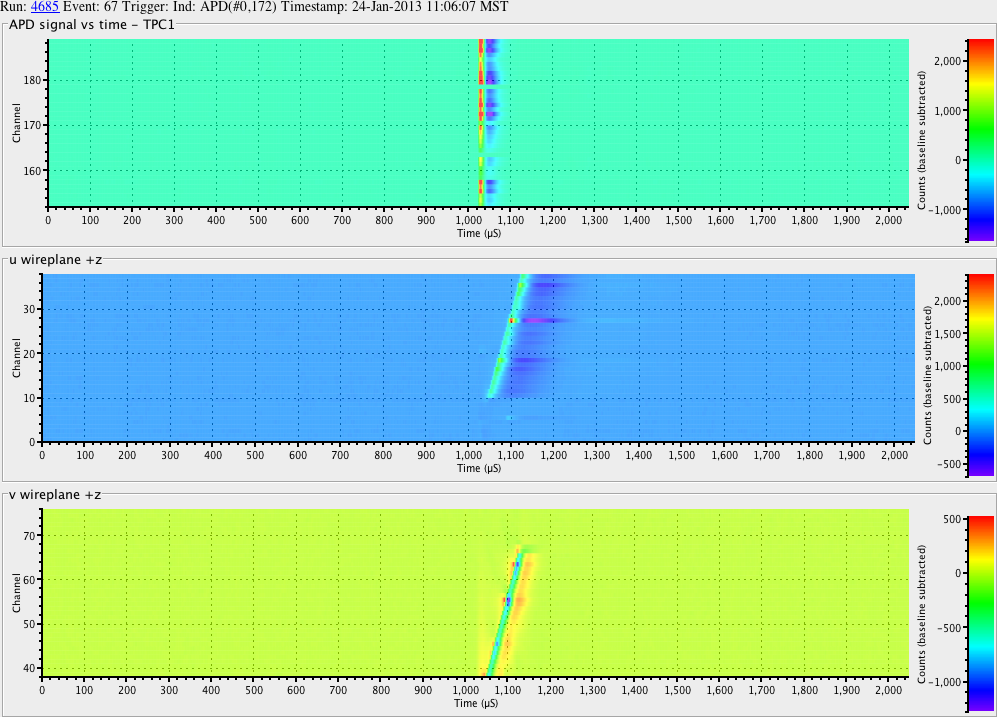
\includegraphics[width=1\columnwidth]{./plots/muon_run_4685_ev_67.png}
\caption[A muon passing through EXO-200]{The event display for a muon passing through EXO-200. The upper panel shows the APDs versus time, displaying the flash of light when the muon passes through. The middle (lower) panel shows u (v) wire channels versus time, showing the characteristic linear trail of ionization.}
\label{fig:muon:eventdisplay}
\end{figure}

\subsection{Hough Transform}



For a particle incident from zenith angle \(\theta\) and azimuthal angle \(\phi\), the effective area of a cylinder on its side is
\begin{equation}
A(\theta,\phi) = \pi r^2 |\cos(\phi)|\sin(\theta) + 2 r h \sqrt{1-\sin(\theta)^2 \cos(\phi)^2}
\end{equation}
when \(\phi=0\) is parallel to the cylinder's axis and where \(r\) is the cylinder's radius and \(h\) is its height.

\end{document} 